\documentclass[aspectratio=169]{beamer}
\usetheme{Madrid}
\usecolortheme{default}

% 包和设置
\usepackage[utf8]{inputenc}
\usepackage[T1]{fontenc}
\usepackage{amsmath,amssymb,amsfonts}
\usepackage{graphicx}
\usepackage{booktabs}
\usepackage{multirow}
\usepackage{tikz}
\usepackage{pgfplots}
\usepackage{xcolor}

% 自定义颜色
\definecolor{zjutblue}{RGB}{0,82,155}
\definecolor{zjutred}{RGB}{220,20,60}
\definecolor{zjutgreen}{RGB}{34,139,34}

% 设置主题颜色
\setbeamercolor{structure}{fg=zjutblue}
\setbeamercolor{frametitle}{bg=zjutblue,fg=white}
\setbeamercolor{title}{fg=zjutblue}

% 标题信息
\title[GRCR-Net]{GRCR-Net: A Complex Residual Network with GPR Denoising and Rotational Augmentation for Automatic Modulation Classification}
\subtitle{突破性的自动调制分类方法}
\author[李俊凯]{李俊凯}
\institute[ZJUT]{浙江工业大学 信息工程学院}
\date{\today}

% 开始文档
\begin{document}

% 标题页
\begin{frame}
\titlepage
\end{frame}

% 目录
\begin{frame}{目录}
\tableofcontents
\end{frame}

% 第一部分:研究背景与挑战
\section{研究背景与挑战}

\begin{frame}{自动调制分类的重要性}
\begin{columns}
\begin{column}{0.6\textwidth}
\begin{itemize}
\item \textbf{认知无线电}:动态频谱感知与管理
\item \textbf{频谱监测}:无线电环境态势感知
\item \textbf{军事通信}:电子对抗与信号情报
\item \textbf{5G/6G通信}:智能信号处理
\end{itemize}
\end{column}
\begin{column}{0.4\textwidth}
\begin{tikzpicture}[scale=0.8]
\node[draw,circle,fill=zjutblue!20] (amc) at (0,0) {AMC};
\node[draw,rectangle,fill=zjutgreen!20] (cr) at (-1.5,1.5) {认知无线电};
\node[draw,rectangle,fill=zjutgreen!20] (sm) at (1.5,1.5) {频谱监测};
\node[draw,rectangle,fill=zjutgreen!20] (mc) at (-1.5,-1.5) {军事通信};
\node[draw,rectangle,fill=zjutgreen!20] (ic) at (1.5,-1.5) {智能通信};
\draw[->] (amc) -- (cr);
\draw[->] (amc) -- (sm);
\draw[->] (amc) -- (mc);
\draw[->] (amc) -- (ic);
\end{tikzpicture}
\end{column}
\end{columns}
\end{frame}

\begin{frame}{核心挑战:低信噪比环境下的性能下降}
\begin{columns}
\begin{column}{0.5\textwidth}
\textbf{传统方法的局限性:}
\begin{itemize}
\item 基于似然的方法计算复杂度高
\item 基于特征的方法依赖专家知识
\item 深度学习方法在低SNR下性能急剧下降
\end{itemize}

\vspace{0.5cm}
\textbf{关键问题:}
\begin{itemize}
\item 噪声严重影响信号质量
\item I/Q信号的相位信息容易丢失
\item 数据不平衡和泛化能力不足
\end{itemize}
\end{column}
\begin{column}{0.5\textwidth}
\begin{tikzpicture}[scale=0.9]
\begin{axis}[
    xlabel={SNR (dB)},
    ylabel={准确率 (\%)},
    grid=major,
    legend pos=south east,
    width=6cm,
    height=4cm
]
\addplot[color=red,mark=square,thick] coordinates {
    (-20,10) (-15,15) (-10,25) (-5,45) (0,65) (5,80) (10,85)
};
\addplot[color=blue,mark=circle,thick] coordinates {
    (-20,9) (-15,35) (-10,51) (-5,78) (0,88) (5,91) (10,93)
};
\legend{传统方法,GRCR-Net}
\end{axis}
\end{tikzpicture}
\end{column}
\end{columns}
\end{frame}

% 第二部分:创新方法概述
\section{GRCR-Net创新方法}

\begin{frame}{GRCR-Net:三大核心创新}
\begin{center}
\begin{tikzpicture}[scale=1.2]
% 主框架
\node[draw,rectangle,fill=zjutblue!20,minimum width=8cm,minimum height=1cm] (main) at (0,0) {\textbf{GRCR-Net 混合架构}};

% 三大创新模块
\node[draw,rectangle,fill=zjutgreen!20,minimum width=2.2cm,minimum height=1.5cm] (gpr) at (-3,-2) {
\begin{minipage}{2cm}
\centering
\textbf{GPR去噪}\\
自适应噪声抑制
\end{minipage}
};

\node[draw,rectangle,fill=zjutred!20,minimum width=2.2cm,minimum height=1.5cm] (aug) at (0,-2) {
\begin{minipage}{2cm}
\centering
\textbf{旋转增强}\\
几何对称性利用
\end{minipage}
};

\node[draw,rectangle,fill=orange!20,minimum width=2.2cm,minimum height=1.5cm] (hybrid) at (3,-2) {
\begin{minipage}{2cm}
\centering
\textbf{混合架构}\\
ComplexCNN+ResNet
\end{minipage}
};

% 连接线
\draw[->] (main) -- (gpr);
\draw[->] (main) -- (aug);
\draw[->] (main) -- (hybrid);

% 性能提升标注
\node[fill=yellow!30] at (-3,-3.2) {+5.86\%};
\node[fill=yellow!30] at (0,-3.2) {+3.78\%};
\node[fill=yellow!30] at (3,-3.2) {+8.27\%};
\end{tikzpicture}
\end{center}

\vspace{0.5cm}
\begin{center}
\textcolor{zjutred}{\textbf{最终性能:65.38\% 准确率,超越现有SOTA方法}}
\end{center}
\end{frame}

% 第三部分:技术细节
\section{核心技术详解}

\begin{frame}{创新一:自适应GPR去噪算法}
\begin{columns}
\begin{column}{0.6\textwidth}
\textbf{核心思想:}
\begin{itemize}
\item 基于信噪比的自适应噪声估计
\item 动态调整核函数长度尺度
\item 分别处理I/Q两个通道
\end{itemize}

\textbf{数学原理:}
\begin{align}
\sigma_n &= \sqrt{\frac{P_r}{2(10^{SNR_{dB}/10}+1)}} \\
L &= \max(L_{min}, L_0(1+SNR/20))
\end{align}

\textbf{关键优势:}
\begin{itemize}
\item 低SNR条件下提升7.25个百分点
\item 保持信号特征完整性
\item 计算效率高
\end{itemize}
\end{column}
\begin{column}{0.4\textwidth}
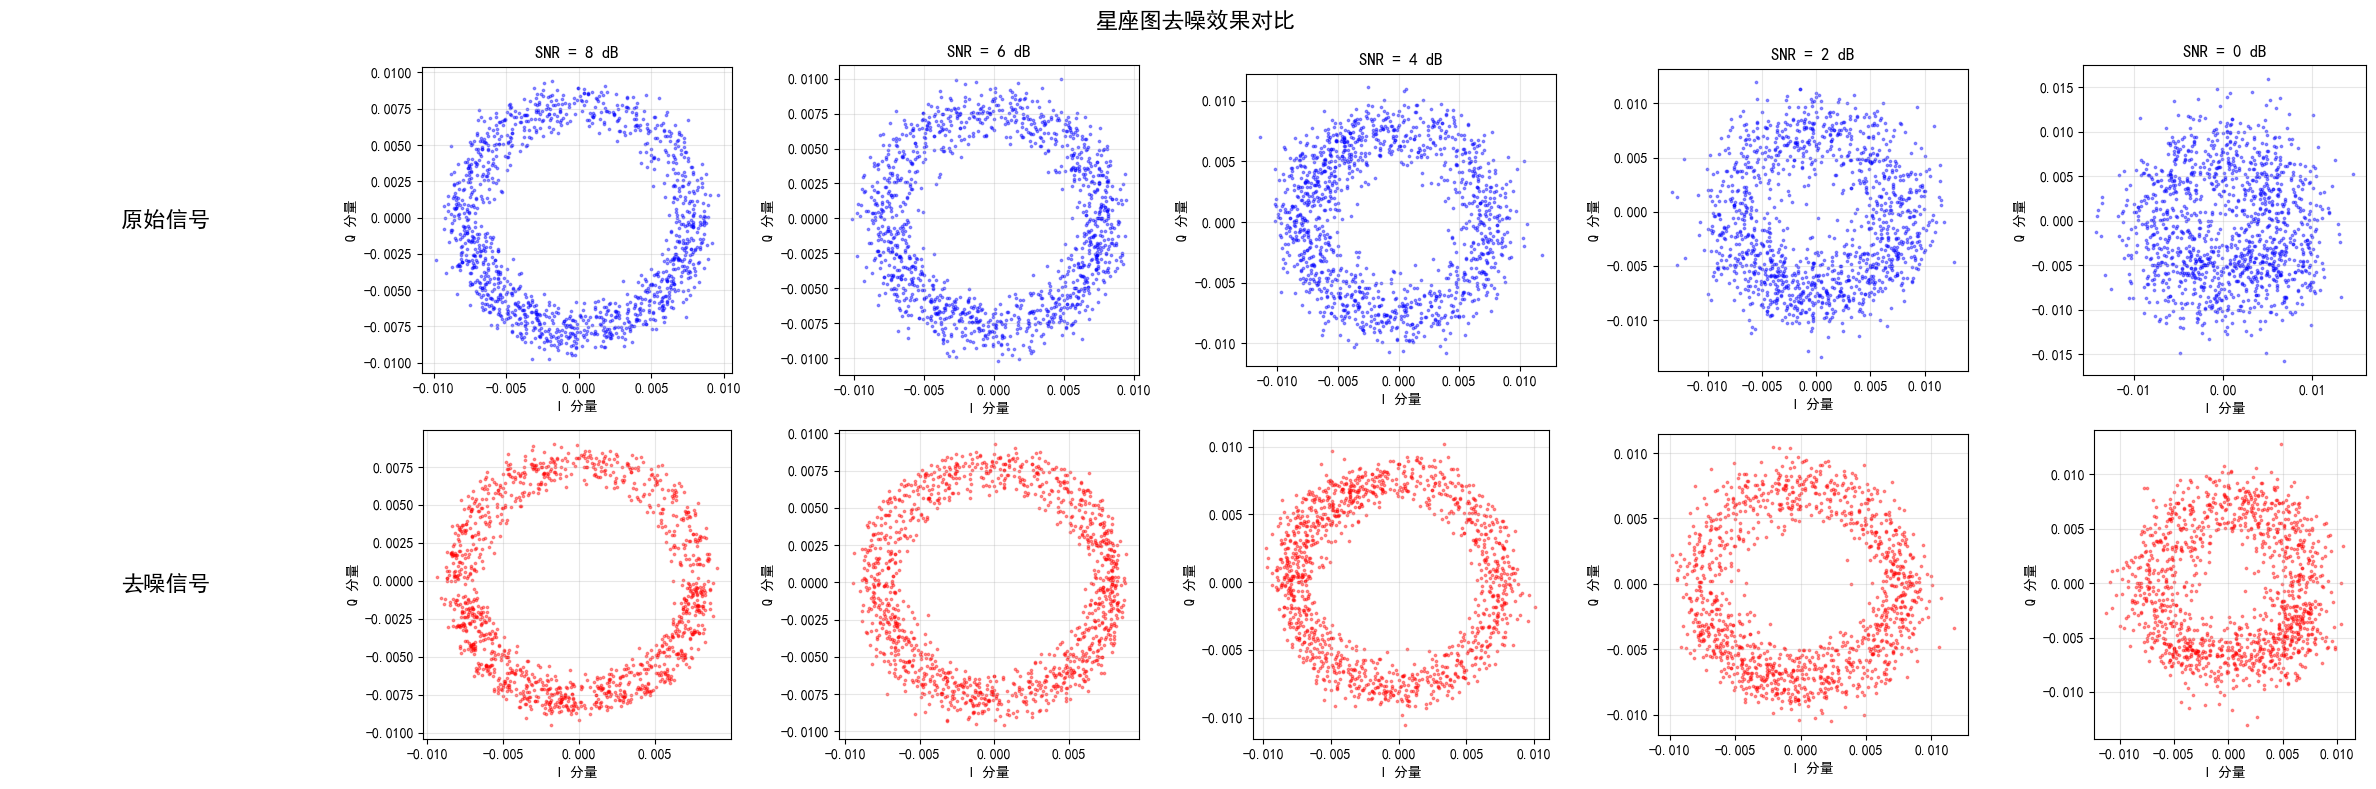
\includegraphics[width=\textwidth]{../paper/figure/constellation_denoising.png}
\end{column}
\end{columns}
\end{frame}

\begin{frame}{创新二:基于几何对称性的旋转数据增强}
\begin{columns}
\begin{column}{0.5\textwidth}
\textbf{理论基础:}
\begin{itemize}
\item 数字调制信号星座图的旋转对称性
\item 复平面旋转变换的数学严格性
\item 相位不变性的利用
\end{itemize}

\textbf{实现方法:}
\begin{equation}
\begin{bmatrix} s'_I[n] \\ s'_Q[n] \end{bmatrix} = \begin{bmatrix} \cos\theta & -\sin\theta \\ \sin\theta & \cos\theta \end{bmatrix} \begin{bmatrix} s_I[n] \\ s_Q[n] \end{bmatrix}
\end{equation}

\textbf{增强策略:}
\begin{itemize}
\item 90°, 180°, 270°旋转
\item 训练数据扩充4倍
\item 针对对称调制类型
\end{itemize}
\end{column}
\begin{column}{0.5\textwidth}
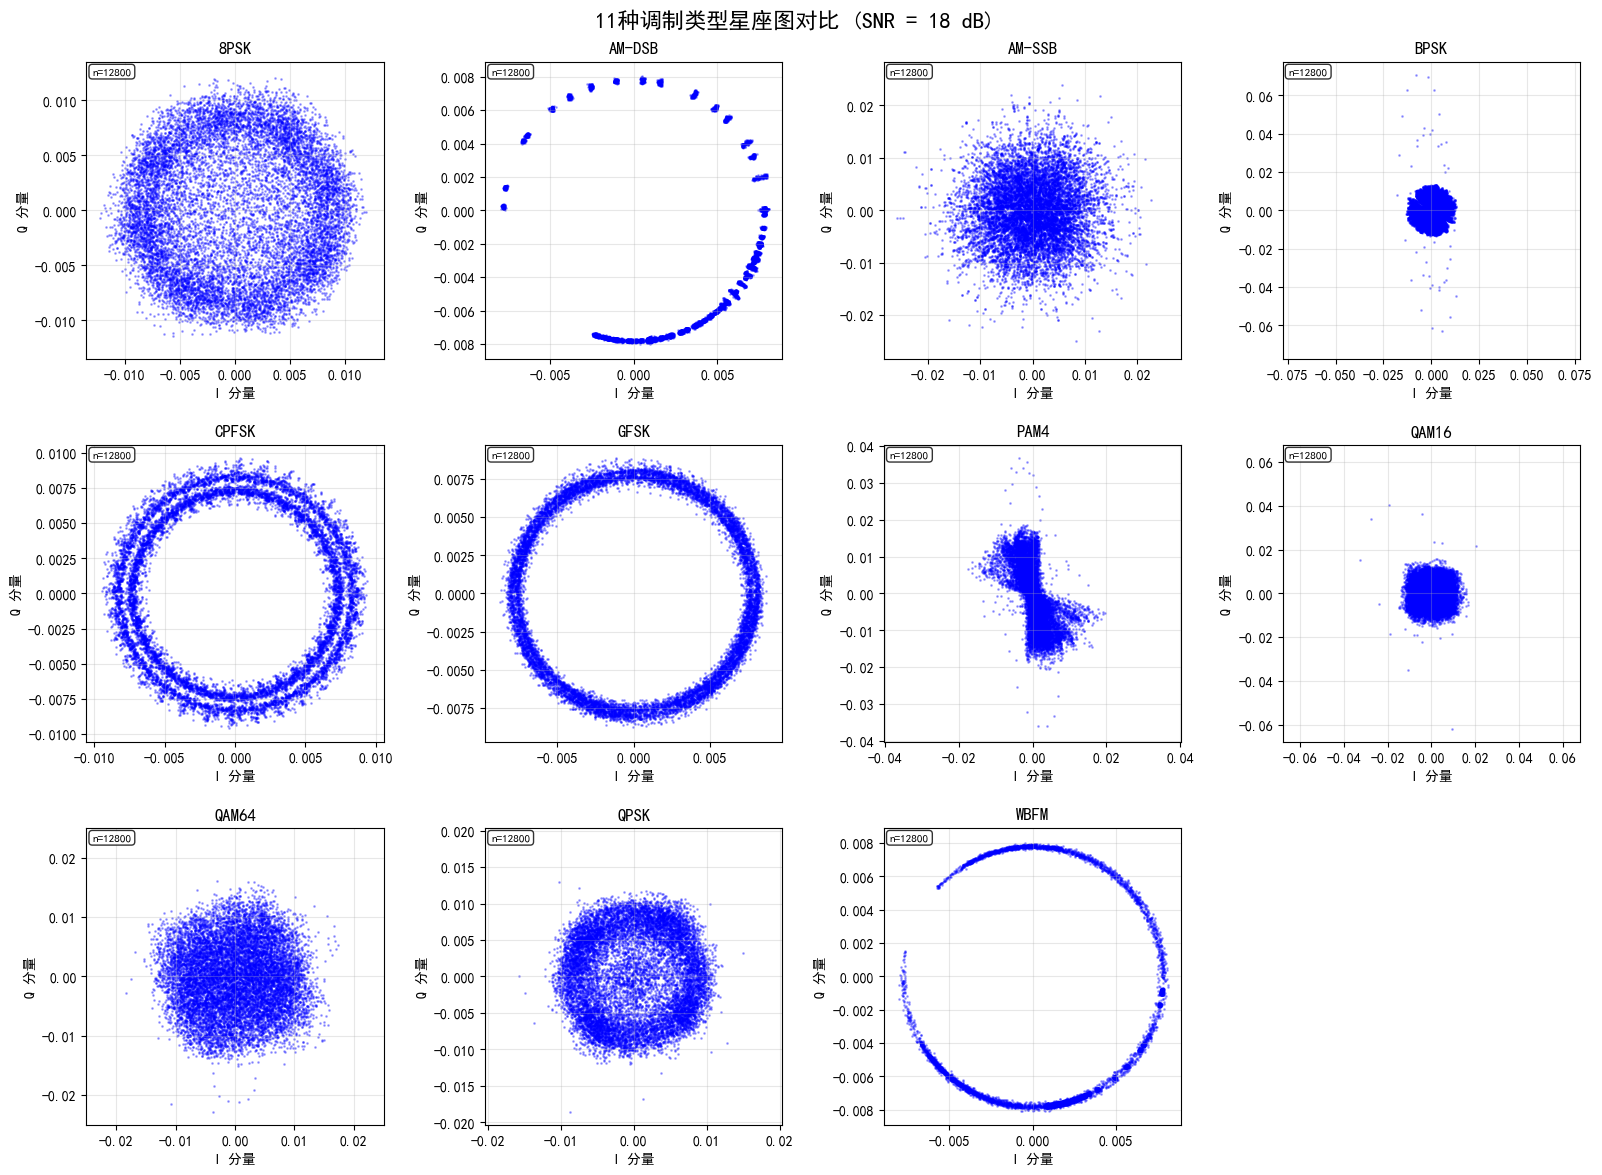
\includegraphics[width=\textwidth]{../paper/figure/constellation.png}
\end{column}
\end{columns}
\end{frame}

\begin{frame}{创新三:混合ComplexCNN-ResNet架构}
\begin{center}
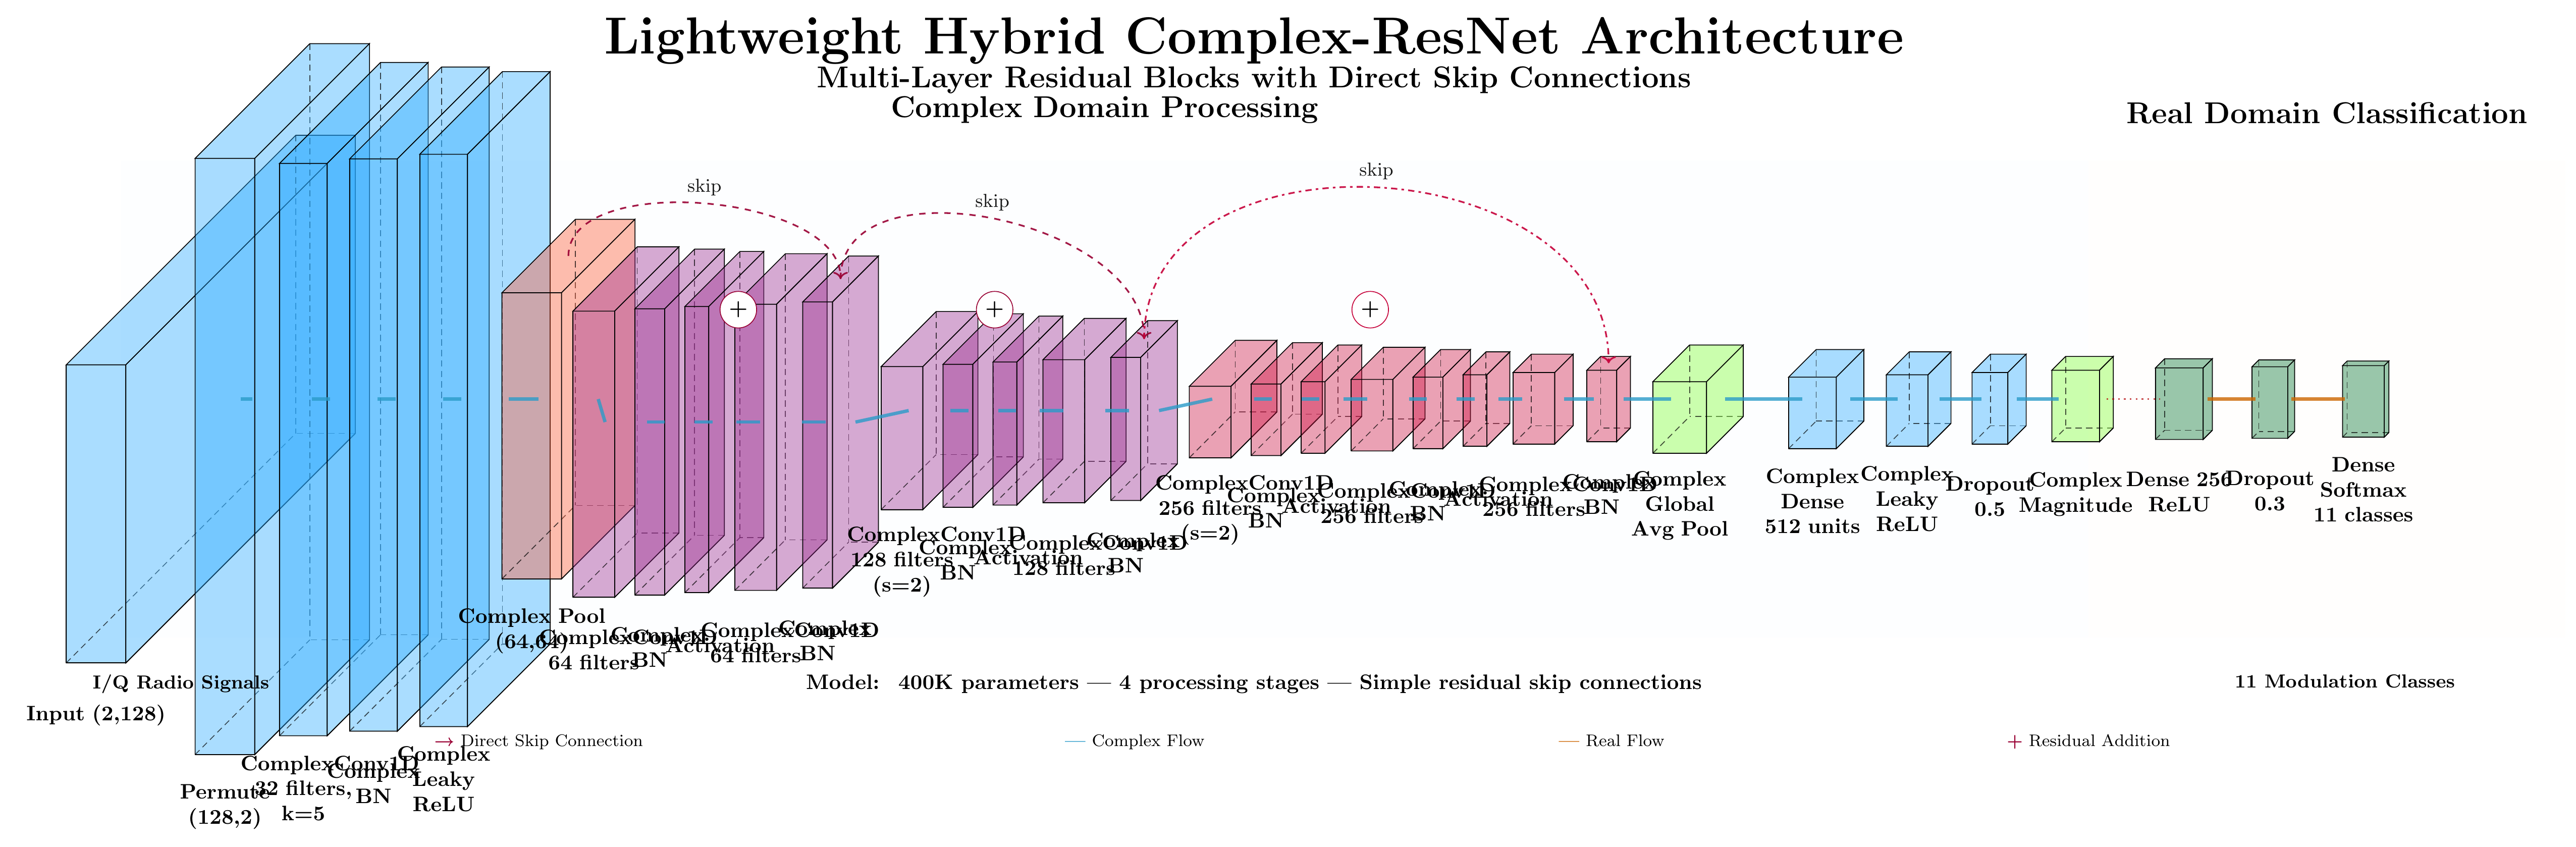
\includegraphics[width=0.9\textwidth]{../paper/figure/enhanced_hybrid_model.pdf}
\end{center}

\textbf{设计原理:}
\begin{itemize}
\item \textbf{复数域处理}:直接处理I/Q信号,保持相位信息
\item \textbf{残差学习}:解决深层网络梯度消失问题
\item \textbf{ModReLU激活}:保持复数几何结构
\item \textbf{轻量化设计}:平衡性能与计算效率
\end{itemize}

\end{frame}

% 第四部分:实验结果
\section{实验结果与分析}

\begin{frame}{数据集与实验设置}
\begin{columns}
\begin{column}{0.6\textwidth}
\textbf{RML2016.10a数据集:}
\begin{itemize}
\item 11种调制类型
\item SNR范围:-20dB到+18dB
\item 每个样本128个复数采样点
\item 数据分割:72\%/8\%/20\%
\end{itemize}

\textbf{实验环境:}
\begin{itemize}
\item Intel Core i9-13900K
\item NVIDIA GeForce RTX 4090 (24GB)
\item TensorFlow 2.17.0 + Keras 3.6.0
\item Ubuntu 24.04.2 LTS
\end{itemize}
\end{column}
\begin{column}{0.4\textwidth}
\begin{table}[h]
\centering
\scriptsize
\begin{tabular}{@{}cc@{}}
\toprule
调制类型 & 样本数 \\
\midrule
8PSK & 22,000 \\
AM-DSB & 22,000 \\
AM-SSB & 22,000 \\
BPSK & 22,000 \\
CPFSK & 22,000 \\
GFSK & 22,000 \\
PAM4 & 22,000 \\
QAM16 & 22,000 \\
QAM64 & 22,000 \\
QPSK & 22,000 \\
WBFM & 22,000 \\
\bottomrule
\end{tabular}
\end{table}
\end{column}
\end{columns}
\end{frame}

\begin{frame}{基线模型性能对比}
\begin{columns}
\begin{column}{0.5\textwidth}
\begin{table}[h]
\centering
\begin{tabular}{@{}cc@{}}
\toprule
\textbf{模型架构} & \textbf{准确率 (\%)} \\
\midrule
FCNN & 42.65 \\
CNN2D & 47.31 \\
Transformer & 47.86 \\
CNN1D & 54.94 \\
ResNet & 55.37 \\
ComplexCNN & 57.11 \\
\midrule
\textcolor{zjutred}{\textbf{GRCR-Net}} & \textcolor{zjutred}{\textbf{65.38}} \\
\bottomrule
\end{tabular}
\end{table}
\end{column}
\begin{column}{0.5\textwidth}
\textbf{关键发现:}
\begin{itemize}
\item ComplexCNN在处理I/Q信号方面具有天然优势
\item ResNet的残差连接有效改善训练稳定性
\item \textcolor{zjutred}{\textbf{GRCR-Net相比最佳基线提升8.27个百分点}}
\end{itemize}

\vspace{0.5cm}
\textbf{性能突破:}
\begin{itemize}
\item 超越现有SOTA方法
\item 在所有SNR条件下均有提升
\item 特别在低SNR环境下表现卓越
\end{itemize}
\end{column}
\end{columns}
\end{frame}

\begin{frame}{消融实验:各组件贡献分析}
\begin{center}
\begin{tikzpicture}[scale=1.1]
\begin{axis}[
    ybar,
    bar width=0.6cm,
    xlabel={方法组合},
    ylabel={准确率 (\%)},
    symbolic x coords={基线,+GPR,+增强,+GPR+增强},
    xtick=data,
    ymin=50,
    ymax=70,
    grid=major,
    width=10cm,
    height=6cm,
    nodes near coords,
    nodes near coords align={vertical},
]
\addplot[fill=zjutblue!50] coordinates {
    (基线,56.94)
    (+GPR,62.80)
    (+增强,60.72)
    (+GPR+增强,65.38)
};
\end{axis}
\end{tikzpicture}
\end{center}

\textbf{关键洞察:}
\begin{itemize}
\item GPR去噪贡献最大:+5.86个百分点
\item 旋转增强提供稳定改进:+3.78个百分点
\item 两种技术协同效应显著:总提升8.44个百分点
\end{itemize}
\end{frame}

\begin{frame}{不同SNR条件下的性能表现}
\begin{center}
\begin{tikzpicture}[scale=1.0]
\begin{axis}[
    xlabel={SNR (dB)},
    ylabel={准确率 (\%)},
    grid=major,
    legend pos=south east,
    width=12cm,
    height=6cm,
    xmin=-20,
    xmax=18,
    ymin=0,
    ymax=100
]
\addplot[color=red,mark=square,thick,mark size=2pt] coordinates {
    (-20,8.93) (-18,8.68) (-16,9.85) (-14,11.08) (-12,12.65) (-10,20.15)
    (-8,34.66) (-6,54.86) (-4,64.02) (-2,75.66) (0,79.43) (2,82.96)
    (4,84.56) (6,83.93) (8,83.17) (10,84.73) (12,85.81) (14,85.31)
    (16,82.25) (18,83.87)
};
\addplot[color=zjutblue,mark=circle,thick,mark size=2pt] coordinates {
    (-20,9.65) (-18,10.08) (-16,13.21) (-14,19.31) (-12,24.72) (-10,35.05)
    (-8,50.62) (-6,64.05) (-4,77.84) (-2,85.73) (0,87.80) (2,91.44)
    (4,91.39) (6,92.63) (8,91.54) (10,91.53) (12,93.37) (14,92.27)
    (16,91.35) (18,91.25)
};
\legend{基线混合架构,GRCR-Net}
\end{axis}
\end{tikzpicture}
\end{center}

\textbf{性能亮点:}
\begin{itemize}
\item 低SNR(-20dB到-8dB):平均提升7.25个百分点
\item 中SNR(-6dB到4dB):平均提升5.12个百分点
\item 高SNR(6dB到18dB):平均提升5.07个百分点
\end{itemize}
\end{frame}

% 第五部分:技术贡献与影响
\section{技术贡献与影响}

\begin{frame}{主要技术贡献}
\begin{enumerate}
\item \textbf{自适应噪声抑制技术}
\begin{itemize}
\item 首次提出基于SNR自适应的GPR去噪算法
\item 实现不同噪声条件下的最优去噪效果
\item 为复杂电磁环境下的信号处理提供新思路
\end{itemize}

\item \textbf{几何特性数据增强策略}
\begin{itemize}
\item 充分利用调制信号的内在对称性
\item 显著提升模型对相位偏移的鲁棒性
\item 为数据稀缺场景提供有效解决方案
\end{itemize}

\item \textbf{混合神经网络架构创新}
\begin{itemize}
\item 首次融合ComplexCNN与ResNet优势
\item 在复数域实现深度残差学习
\item 为I/Q信号处理提供新的架构范式
\end{itemize}
\end{enumerate}
\end{frame}

\begin{frame}{与现有方法的对比优势}
\begin{table}[h]
\centering
\scriptsize
\begin{tabular}{@{}lccc@{}}
\toprule
\textbf{方法} & \textbf{准确率(\%)} & \textbf{参数量} & \textbf{特色技术} \\
\midrule
AMC-Net & 62.51 & 较大 & 频域去噪 \\
AbFTNet & 64.59 & 较大 & 多模态融合 \\
HFECNET-CA & 约60 & 小 & 注意力机制 \\
LDCVNN & 约58 & 小 & 双分支复数网络 \\
\midrule
\textcolor{zjutred}{\textbf{GRCR-Net}} & \textcolor{zjutred}{\textbf{65.38}} & \textcolor{zjutred}{\textbf{中等}} & \textcolor{zjutred}{\textbf{GPR+旋转+混合架构}} \\
\bottomrule
\end{tabular}
\end{table}

\vspace{0.5cm}
\textbf{核心优势:}
\begin{itemize}
\item \textcolor{zjutgreen}{\textbf{性能领先}}:超越现有最佳方法0.79个百分点
\item \textcolor{zjutgreen}{\textbf{技术创新}}:三大核心技术的有机融合
\item \textcolor{zjutgreen}{\textbf{实用性强}}:在复杂环境下表现稳定
\item \textcolor{zjutgreen}{\textbf{可扩展性}}:技术组件可独立应用
\end{itemize}
\end{frame}

\begin{frame}{实际应用价值与前景}
\begin{columns}
\begin{column}{0.6\textwidth}
\textbf{直接应用领域:}
\begin{itemize}
\item \textbf{认知无线电}:智能频谱感知与管理
\item \textbf{电子对抗}:信号侦察与识别
\item \textbf{通信监管}:频谱监测与合规检查
\item \textbf{5G/6G网络}:智能信号处理
\end{itemize}

\textbf{技术扩展价值:}
\begin{itemize}
\item GPR去噪技术可应用于其他信号处理任务
\item 混合架构思想可推广到其他复数信号分析
\item 旋转增强策略适用于具有几何对称性的数据
\end{itemize}
\end{column}
\begin{column}{0.4\textwidth}
\begin{tikzpicture}[scale=0.8]
% 应用场景图
\node[draw,circle,fill=zjutblue!20] (core) at (0,0) {GRCR-Net};
\node[draw,rectangle,fill=zjutgreen!20,text width=1.5cm,align=center] (cr) at (-2,2) {认知\\无线电};
\node[draw,rectangle,fill=zjutgreen!20,text width=1.5cm,align=center] (ew) at (2,2) {电子\\对抗};
\node[draw,rectangle,fill=zjutgreen!20,text width=1.5cm,align=center] (sm) at (-2,-2) {频谱\\监管};
\node[draw,rectangle,fill=zjutgreen!20,text width=1.5cm,align=center] (ng) at (2,-2) {下一代\\通信};

\draw[->] (core) -- (cr);
\draw[->] (core) -- (ew);
\draw[->] (core) -- (sm);
\draw[->] (core) -- (ng);
\end{tikzpicture}
\end{column}
\end{columns}
\end{frame}

% 第六部分:总结与展望
\section{总结与展望}

\begin{frame}{研究总结}
\begin{center}
\textcolor{zjutblue}{\Large \textbf{GRCR-Net:突破性的自动调制分类方法}}
\end{center}

\vspace{0.5cm}
\begin{columns}
\begin{column}{0.5\textwidth}
\textbf{核心成就:}
\begin{itemize}
\item ✅ 达到65.38\%的分类准确率
\item ✅ 超越现有SOTA方法
\item ✅ 在低SNR环境下表现卓越
\item ✅ 提出三大核心技术创新
\end{itemize}

\textbf{技术突破:}
\begin{itemize}
\item 🔬 自适应GPR去噪算法
\item 🔄 几何对称性数据增强
\item 🏗️ 混合ComplexCNN-ResNet架构
\end{itemize}
\end{column}
\begin{column}{0.5\textwidth}
\textbf{影响意义:}
\begin{itemize}
\item 🎯 为复杂电磁环境提供解决方案
\item 🚀 推动认知无线电技术发展
\item 💡 为信号处理领域提供新思路
\item 🌟 具有重要的理论与实践价值
\end{itemize}

\textbf{开源贡献:}
\begin{itemize}
\item 📂 完整代码开源
\item 📊 详细实验数据
\item 📖 技术文档完善
\end{itemize}
\end{column}
\end{columns}
\end{frame}

\begin{frame}{未来研究方向}
\begin{enumerate}
\item \textbf{算法优化与扩展}
\begin{itemize}
\item 探索更复杂信道环境下的性能
\item 研究实时处理的优化策略
\item 扩展到更多调制类型
\end{itemize}

\item \textbf{技术融合与创新}
\begin{itemize}
\item 结合Transformer等新兴架构
\item 探索多模态信号融合
\item 研究自监督学习方法
\end{itemize}

\item \textbf{实际部署与应用}
\begin{itemize}
\item 硬件加速与边缘计算优化
\item 大规模实际环境验证
\item 产业化应用推广
\end{itemize}
\end{enumerate}
\end{frame}

\begin{frame}[standout]
\centering
\Huge \textcolor{white}{\textbf{谢谢聆听!}}

\vspace{1cm}
\Large \textcolor{white}{欢迎提问与交流}

\vspace{1cm}
\normalsize
\textcolor{white}{
代码开源地址:\\
\url{https://github.com/LJK666666666/radioML-v3}
}
\end{frame}

\end{document}
